% 第 8 题图乙：A、B 两物体的 a-t 图像（示意曲线）
% S1：0~t1 内 A 的图线与轴围成面积；S2：t1~t2 内 A；S3：t1~t2 内 B。
% 曲线形状为示意：A 先正后负（t2 时刻加速度最大），B 在 t1 后从 0 增大（t2 时刻最大）。
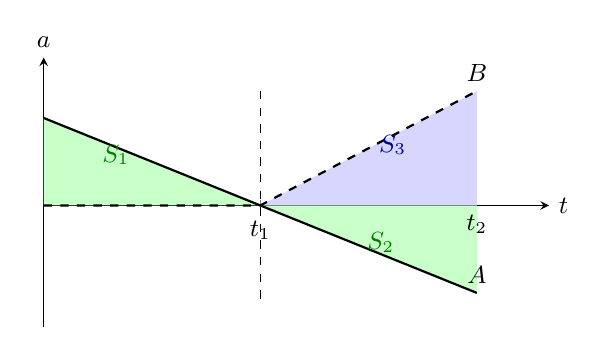
\begin{tikzpicture}[font=\small]
  \def\T{3.6}  % t2
  \def\T1{1.8} % t1
  \begin{axis}[
      width=8cm, height=5cm, axis lines=middle,
      xlabel={$t$}, ylabel={$a$}, xmin=0, xmax=4.2, ymin=-1.8, ymax=2.2,
      xtick={1.8}, xticklabels={$t_1$}, ytick=\empty, xlabel style={anchor=west},
      ylabel style={anchor=south}, font=\small]
    % S1：0~t1 内 A 的 a-t 面积（正值区域，阴影）
    \fill[green!30, opacity=0.7] (0,1.3) -- (1.8,0) -- (0,0) -- cycle;
    % S2：t1~t2 内 A 的面积（负值区域，阴影）
    \fill[green!30, opacity=0.7] (1.8,0) -- (3.6,-1.3) -- (3.6,0) -- cycle;
    % S3：t1~t2 内 B 的面积（正值区域，阴影）
    \fill[blue!20, opacity=0.8] (1.8,0) -- (3.6,1.7) -- (3.6,0) -- cycle;
    % A 曲线：0~t1 正值降为 0，t1~t2 变为负值且幅值增大
    \addplot[thick] coordinates {(0,1.3) (1.8,0) (3.6,-1.3)};
    % B 曲线：t1 前为 0，t1~t2 正值增大
    \addplot[thick, dashed] coordinates {(0,0) (1.8,0) (3.6,1.7)};
    \node[green!50!black] at (0.6,0.75) {$S_{1}$};
    \node[green!50!black] at (2.8,-0.55) {$S_{2}$};
    \node[blue!60!black] at (2.9,0.9) {$S_{3}$};
    \node[above] at (3.6,-1.3) {$A$};
    \node[above] at (3.6,1.7) {$B$};
    \draw[dashed] (1.8,1.7) -- (1.8,-1.4);
    \node[below] at (3.6,0) {$t_2$};
  \end{axis}
\end{tikzpicture}
